\section{Structures des systèmes automatisés}

\begin{figure}[ht]
	\centering
	


\tikzset{every picture/.style={line width=0.75pt}} %set default line width to 0.75pt

\begin{tikzpicture}[x=0.75pt,y=0.75pt,yscale=-1,xscale=1]
%uncomment if require: \path (0,300); %set diagram left start at 0, and has height of 300

%Rounded Rect [id:dp6996926995502989]
\draw   (86,94.6) .. controls (86,87.09) and (92.09,81) .. (99.6,81) -- (317.4,81) .. controls (324.91,81) and (331,87.09) .. (331,94.6) -- (331,135.4) .. controls (331,142.91) and (324.91,149) .. (317.4,149) -- (99.6,149) .. controls (92.09,149) and (86,142.91) .. (86,135.4) -- cycle ;
%Image [id:dp5199524107849971]
\draw (302.2,113.2) node  {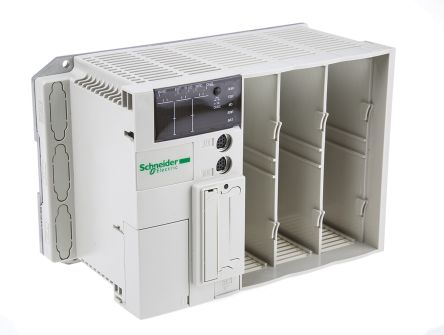
\includegraphics[width=43.2pt,height=43.2pt]{images/automate_schneider.jpg}};
%Rounded Rect [id:dp4357143022979344]
\draw  [fill={rgb, 255:red, 255; green, 245; blue, 245 }  ,fill opacity=1 ][line width=0.75]  (20.83,194.2) .. controls (20.83,181.39) and (31.21,171) .. (44.03,171) -- (372.97,171) .. controls (385.79,171) and (396.17,181.39) .. (396.17,194.2) -- (396.17,263.8) .. controls (396.17,276.61) and (385.79,287) .. (372.97,287) -- (44.03,287) .. controls (31.21,287) and (20.83,276.61) .. (20.83,263.8) -- cycle ;
%Rounded Rect [id:dp8390570092351776]
\draw  [color={rgb, 255:red, 208; green, 2; blue, 27 }  ,draw opacity=1 ][line width=1.5]  (40,189) .. controls (40,184.58) and (43.58,181) .. (48,181) -- (102,181) .. controls (106.42,181) and (110,184.58) .. (110,189) -- (110,213) .. controls (110,217.42) and (106.42,221) .. (102,221) -- (48,221) .. controls (43.58,221) and (40,217.42) .. (40,213) -- cycle ;
%Rounded Rect [id:dp9242421121217611]
\draw  [color={rgb, 255:red, 65; green, 117; blue, 5 }  ,draw opacity=1 ][line width=1.5]  (274,191) .. controls (274,186.58) and (277.58,183) .. (282,183) -- (380,183) .. controls (384.42,183) and (388,186.58) .. (388,191) -- (388,215) .. controls (388,219.42) and (384.42,223) .. (380,223) -- (282,223) .. controls (277.58,223) and (274,219.42) .. (274,215) -- cycle ;
%Rounded Rect [id:dp5921159806431459]
\draw  [line width=0.75]  (157,229) .. controls (157,224.58) and (160.58,221) .. (165,221) -- (252,221) .. controls (256.42,221) and (260,224.58) .. (260,229) -- (260,253) .. controls (260,257.42) and (256.42,261) .. (252,261) -- (165,261) .. controls (160.58,261) and (157,257.42) .. (157,253) -- cycle ;

%Curve Lines [id:da49513234525320104]
\draw [color={rgb, 255:red, 208; green, 2; blue, 27 }  ,draw opacity=1 ]   (48,181) .. controls (43.13,107.87) and (62.97,116.5) .. (85.28,116.05) ;
\draw [shift={(87,116)}, rotate = 537.51] [color={rgb, 255:red, 208; green, 2; blue, 27 }  ,draw opacity=1 ][line width=0.75]    (10.93,-3.29) .. controls (6.95,-1.4) and (3.31,-0.3) .. (0,0) .. controls (3.31,0.3) and (6.95,1.4) .. (10.93,3.29)   ;

%Curve Lines [id:da8679026938428056]
\draw [color={rgb, 255:red, 65; green, 117; blue, 5 }  ,draw opacity=1 ]   (331,112) .. controls (387.43,107.05) and (351.73,129.54) .. (352.95,180.45) ;
\draw [shift={(353,182)}, rotate = 267.8] [color={rgb, 255:red, 65; green, 117; blue, 5 }  ,draw opacity=1 ][line width=0.75]    (10.93,-3.29) .. controls (6.95,-1.4) and (3.31,-0.3) .. (0,0) .. controls (3.31,0.3) and (6.95,1.4) .. (10.93,3.29)   ;

%Curve Lines [id:da11237972281185649]
\draw    (335,223) .. controls (334.01,240.82) and (318.32,243.94) .. (264.64,241.09) ;
\draw [shift={(263,241)}, rotate = 363.12] [color={rgb, 255:red, 0; green, 0; blue, 0 }  ][line width=0.75]    (10.93,-3.29) .. controls (6.95,-1.4) and (3.31,-0.3) .. (0,0) .. controls (3.31,0.3) and (6.95,1.4) .. (10.93,3.29)   ;

%Curve Lines [id:da3503728176891857]
\draw    (157,243) .. controls (61.94,241.04) and (71.56,253.49) .. (71.99,223.87) ;
\draw [shift={(72,222)}, rotate = 450] [color={rgb, 255:red, 0; green, 0; blue, 0 }  ][line width=0.75]    (10.93,-3.29) .. controls (6.95,-1.4) and (3.31,-0.3) .. (0,0) .. controls (3.31,0.3) and (6.95,1.4) .. (10.93,3.29)   ;

%Straight Lines [id:da7532920416250504]
\draw [color={rgb, 255:red, 208; green, 2; blue, 27 }  ,draw opacity=1 ]   (159,80) -- (159,39) ;
\draw [shift={(159,37)}, rotate = 450] [color={rgb, 255:red, 208; green, 2; blue, 27 }  ,draw opacity=1 ][line width=0.75]    (10.93,-3.29) .. controls (6.95,-1.4) and (3.31,-0.3) .. (0,0) .. controls (3.31,0.3) and (6.95,1.4) .. (10.93,3.29)   ;

%Straight Lines [id:da741979851639265]
\draw [color={rgb, 255:red, 74; green, 144; blue, 226 }  ,draw opacity=1 ]   (141,51) -- (141,77) ;
\draw [shift={(141,79)}, rotate = 270] [color={rgb, 255:red, 74; green, 144; blue, 226 }  ,draw opacity=1 ][line width=0.75]    (10.93,-3.29) .. controls (6.95,-1.4) and (3.31,-0.3) .. (0,0) .. controls (3.31,0.3) and (6.95,1.4) .. (10.93,3.29)   ;

%Rounded Rect [id:dp2079891174972378]
\draw  [dash pattern={on 4.5pt off 4.5pt}] (102,27.4) .. controls (102,23.31) and (105.31,20) .. (109.4,20) -- (194.6,20) .. controls (198.69,20) and (202,23.31) .. (202,27.4) -- (202,49.6) .. controls (202,53.69) and (198.69,57) .. (194.6,57) -- (109.4,57) .. controls (105.31,57) and (102,53.69) .. (102,49.6) -- cycle ;
%Rounded Rect [id:dp14823711603822332]
\draw  [dash pattern={on 4.5pt off 4.5pt}] (245,30) .. controls (245,25.58) and (248.58,22) .. (253,22) -- (307,22) .. controls (311.42,22) and (315,25.58) .. (315,30) -- (315,54) .. controls (315,58.42) and (311.42,62) .. (307,62) -- (253,62) .. controls (248.58,62) and (245,58.42) .. (245,54) -- cycle ;

% Text Node
\draw (208.5,276) node [scale=0.9] [align=left] {Partie opérative};
% Text Node
\draw (75,201) node [color={rgb, 255:red, 208; green, 2; blue, 27 }  ,opacity=1 ] [align=left] {Capteurs};
% Text Node
\draw (332,202) node [color={rgb, 255:red, 65; green, 117; blue, 5 }  ,opacity=1 ] [align=left] {Pré-actionneurs};
% Text Node
\draw (209.5,136) node [scale=0.9] [align=left] {Partie commande};
% Text Node
\draw (384,102) node [color={rgb, 255:red, 65; green, 117; blue, 5 }  ,opacity=1 ] [align=left] {commandes};
% Text Node
\draw (43,106) node [color={rgb, 255:red, 208; green, 2; blue, 27 }  ,opacity=1 ] [align=left] {Informations};
% Text Node
\draw (126,43) node [color={rgb, 255:red, 74; green, 144; blue, 226 }  ,opacity=1 ] [align=left] {{\footnotesize ordres}};
% Text Node
\draw (154,29) node [color={rgb, 255:red, 208; green, 2; blue, 27 }  ,opacity=1 ] [align=left] {{\footnotesize Informations}};
% Text Node
\draw (182,47) node [scale=0.9] [align=left] {IHM};
% Text Node
\draw (186,110) node  [align=left] {Automate Programmable};
% Text Node
\draw (280,52) node [scale=0.9] [align=left] {Réseau};
% Text Node
\draw (209,240) node  [align=left] {Actionneurs};


\end{tikzpicture}

	\caption{Sructure d'un système industriel}
	\label{fig:structureAPI}
\end{figure}

\UPSTIaRetenir{%
	L'API (partie commande) communique avec la \textit{partie opérative} en envoyant des \textit{commandes} aux \textbf{\color{green} pré-actionneurs} et en recevant des \textbf{\color{red} informations} de la part des capteurs.%
}



La Figure~\ref{fig:structureAPI} illustre la communication entre l'automate et la partie opérative d'un système. Il aparaît également l'\textbf{I}nterface \textbf{H}omme \textbf{M}achine (\textbf{IHM}) permettant de communiquer avec les utilisateurs ainsi qu'un réseau informatique pour communiquer avec des ordinateurs, d'autres automates ou même tout appareil sur internet.

\subsection{Composition d'un API}
Un \textit{\textbf{A}utomate \textbf{P}rogrammable \textbf{I}ndustriel (\textbf{API})} est un système informatique industriel adapté aux besoins de l'industrie. Sa structure est donc similaire à celle d'un ordinateur personnel (PC) en cela qu'il est composé d'un processeur et de mémoires dédiées à des usages que nous allons développer. 

\begin{UPSTIactivite}[][Structure d'un API]
    Représenter sous forme schématique un automate industriel
    \begin{center}
        \UPSTIprofEleve{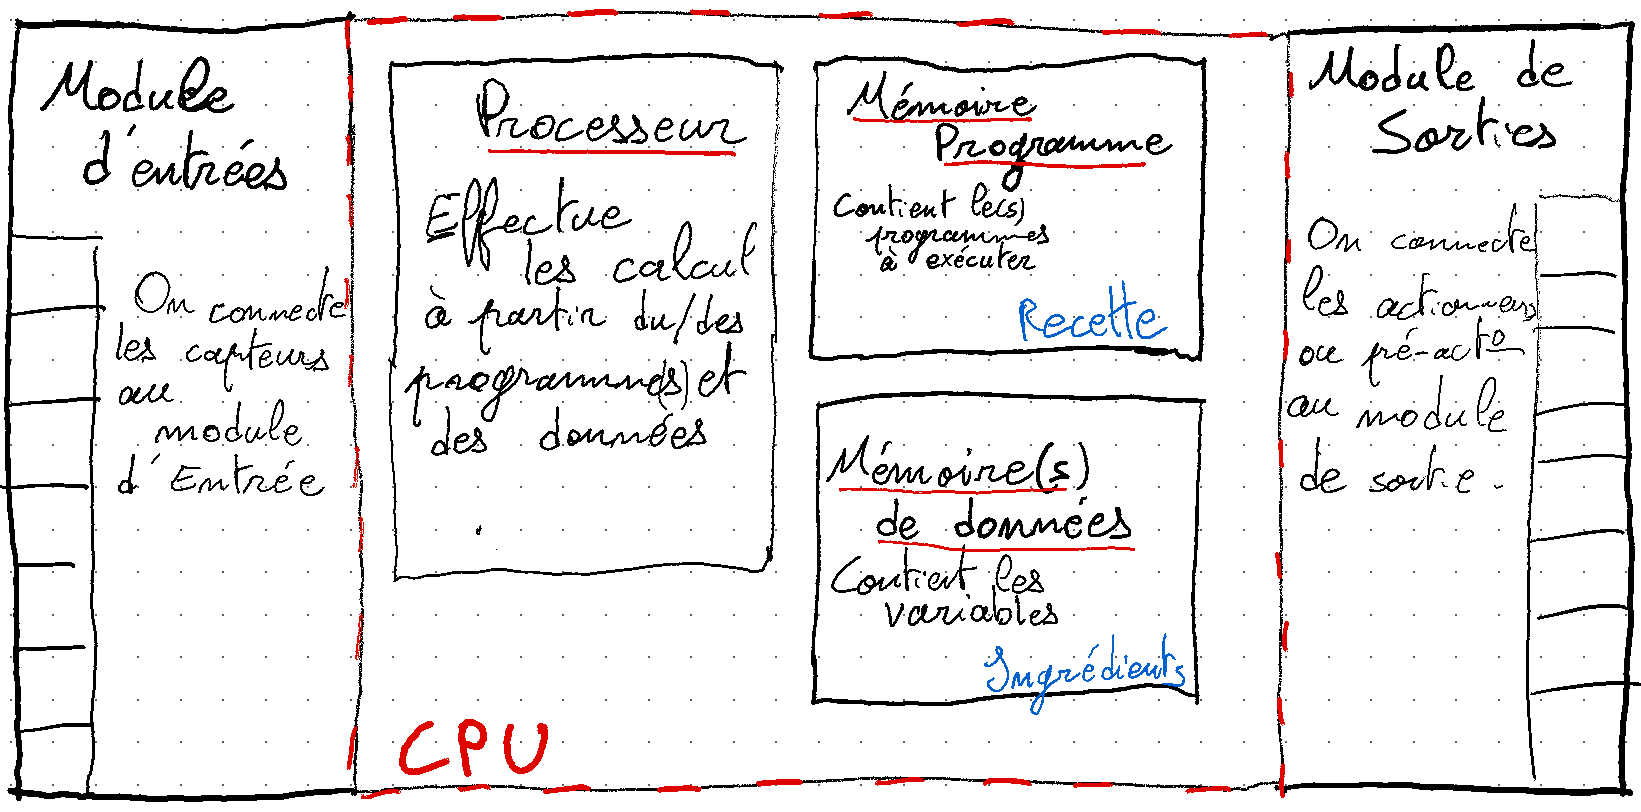
\includegraphics[height=.34\textheight]{images/API}\vspace{.06\textheight}}{\vspace{0.4\textheight}}
    \end{center}   

\end{UPSTIactivite}

Les modules d'entrées-sorties viennent se relier à la CPU en vue de faire le lien avec les capteurs et les actionneurs du système. On qualifie ces automates de \textbf{modulaire} et il est possible d'ajouter un nombre important de module (TOR, analogique, pour sonde de température, etc.) afin d'adapter l'automate aux besoins spécifiques de l'industrie. Un exemple d'automate modulaire \textit{Schneider} est donné en Figure~\ref{fig:schneider}. 

Pour des applications simples, certains constructeurs ont développé des automates \textbf{Monobloc} contenant directement des entrées-sorties sur le bloc de CPU. C'est le cas du LOGO de chez \textit{Siemens} que nous utiliserons en TP (Figure~\ref{fig:logo}). Sur ces automates, il est souvent possible d'ajouter des extension afin de multiplier le nombre d'entrée et de sorties. 

\begin{figure}[ht]
    \centering
    \begin{subfigure}{0.49\textwidth}
        \centering
            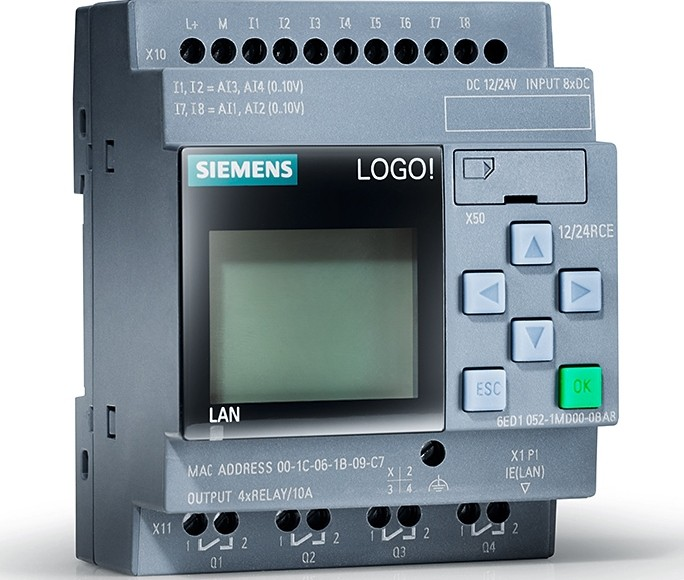
\includegraphics[width=.6\textwidth]{images/logo-v8-siemens}
            \caption{Automate Monobloc : Siemens LOGO}
            \label{fig:logo}
    \end{subfigure}%
    \begin{subfigure}{0.49\textwidth}
        \centering
            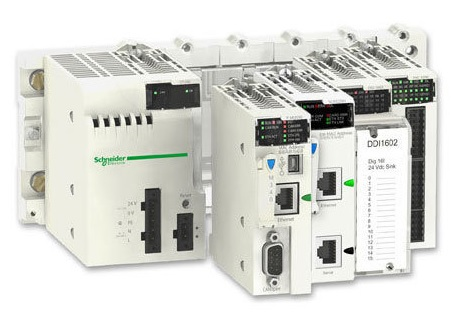
\includegraphics[width=.8\textwidth]{images/api-schneider}
            \caption{Automate Modulaires : Schneider}
            \label{fig:schneider}
    \end{subfigure}%
    \caption{Exemples d'automates monoblocs et modulaires}
\end{figure}

\UPSTIaRetenir{%
Les \textbf{\color{red} capteurs} du système sont reliées aux \textbf{\color{red} modules d'entrées} de l'API.\\
Les \textbf{\color{green} actionneurs} et les \textbf{\color{green} pré-actionneurs}  du système sont reliées aux \textbf{\color{green} modules de sortie} de l'aPI.\\
Les automates \textbf{monoblocs} contiennent des modules d'entrées-sorties incorporé au bloc CPU. À l'inverse, sur un automate \textbf{modulaire} il est nécessaire d'ajouter les modules en fonction des besoin de l'application.}


\subsection{Les capteurs}
Pour exploiter correctement un système automatisé, il est essentiel de \textbf{controler les variations de certaines grandeurs physiques} et \textbf{l'état physique de certains de ses constituants}.

Les capteurs sont des composants permettant d'acquérir une information en provenance du monde extérieur. Dans le cas d'un automate industriel, ils permettent de connaître l'état du système et de mesurer les variations des grandeurs physiques qui lui sont associées.

\UPSTIdefinition{Un capteur transforme une grandeur physique en une grandeur normée, généralement électrique, qui peut être interprétée par un dispositif de contrôle
commande comme l’API.}

\UPSTIaRetenir{Un automate industriel acquiert des informations sur l'état d'un système à l'aide de \textbf{capteurs}}

Il existe trois familles de capteurs se différenciant par la nature du signal qu'ils mesurent :

\begin{description}
	\item [Capteurs Analogiques : ] Le signal délivré est la traduction de la grandeur physique mesurée. Le signal en sortie est généralement sous la forme d'un courant ou d'une tension variable.

	\begin{itemize}
		\item Sonde de température
		\item Capteur de luminosité
		%\item Microphone
		\item Sonde de déformation
		\item \dots
	\end{itemize}

	\item [Capteurs logiques (Tout Ou Rien - TOR) : ] Le signal ne peut prendre que deux valeurs représentant les états 0 et 1. Ces capteurs sont aussi appelés des \textit{détecteurs}.
		\begin{itemize}
			\item Détecteur de proximité
			\item Capteur fin de course de vérin
			\item Détecteur infrarouge
			\item \dots
		\end{itemize}

			\item[Capteurs numériques :] Le signal est codé au sein du capteur. Il est ensuite envoyé sous la forme d'un signal variant de façon discrète dans le temps.
			\begin{itemize}
				\item Codeur d'un moteur
				\item Capteur de température numérique
				\item \dots
			\end{itemize}
\end{description}

La Figure~\ref{fig:analogVsNum} rappelle la forme des signaux analogique et numériques

\begin{figure}[ht]
\centering
\begin{subfigure}{0.49\textwidth}
\centering
	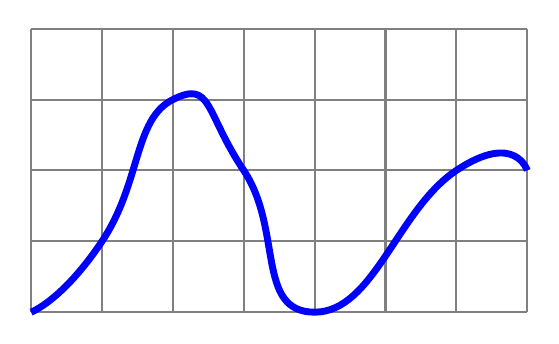
\begin{tikzpicture}[scale = 0.9]
\draw [gray](0,0) grid (7,4);
\draw [blue, line width = 2.5pt] plot [smooth, tension=1] coordinates { (0,0) (1,1) (2,3) (3,2) (4,0) (6,2) (7,2)};
\end{tikzpicture}

	\caption{Signal analogique}
\end{subfigure}%
%
\begin{subfigure}{0.49\textwidth}
\centering
	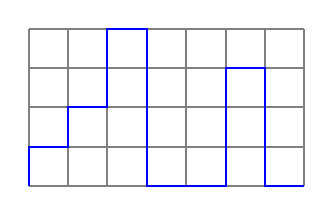
\begin{tikzpicture}[scale = 0.5]
\draw [gray](0,0) grid (7,4);
\draw [blue] plot coordinates { (0,0) (0,1) (1,1) (1,2) (2,2) (2,4) (3,4) (3,0) (5,0) (5,3) (6,3) (6,0) (7,0)};
\end{tikzpicture}

	\caption{Signal numérique}
\end{subfigure}
%
	\caption{Rappel -- signal analogique et numérique}
	\label{fig:analogVsNum}
\end{figure}

\UPSTIremarque[Conversion analogique - numérique]{Il est possible de convertir un signal analogique en un signal numérique. Voir exemple en TD.\\}

\pagebreak
\begin{UPSTIactivite}
\UPSTIquestion{De quel type (analogique, numérique ou logique) sont les capteurs inductif et optique ci-dessous ?}

\UPSTIlignesACompleter[1]{logiques (TOR) car ils ne peuvent prendre que deux valeurs : 1 ou 0.}

	 \begin{minipage}[t]{.45\textwidth}
	\begin{center}
		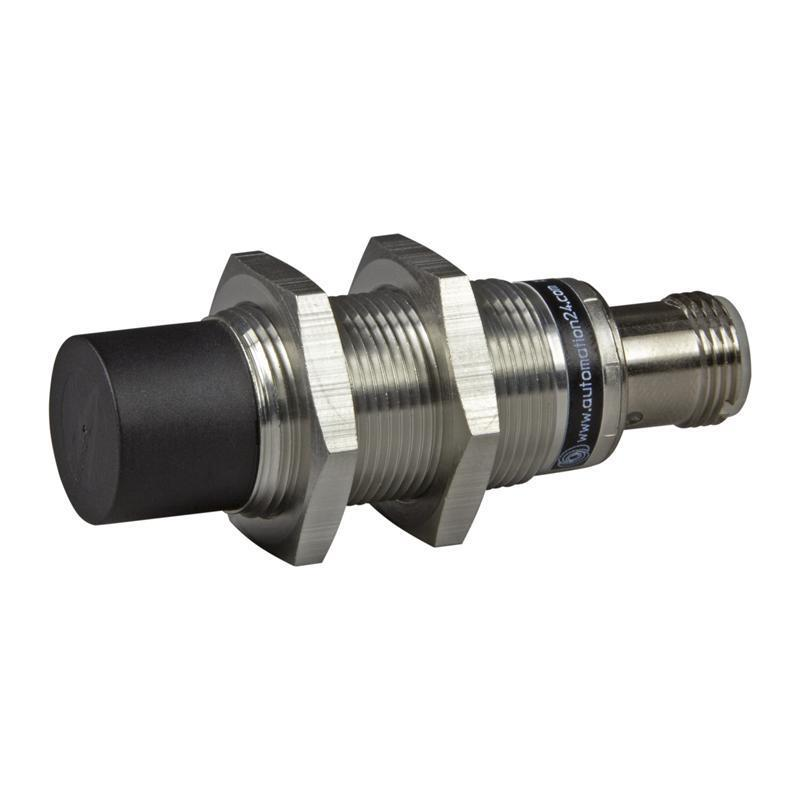
\includegraphics[width=.4\textwidth,height=.4\textheight,keepaspectratio]{images/capt_inductif}
	\end{center}


		Un \textbf{capteur inductif} détecte la présence d'objets métalliques.
	\end{minipage}\hfill
	\begin{minipage}[t]{.45\textwidth}
	\begin{center}
		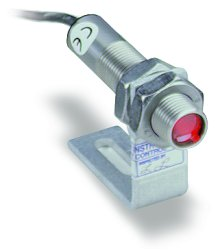
\includegraphics[width=.4\textwidth,height=.3\textheight,keepaspectratio]{images/capt_optique}
	\end{center}
		Un \textbf{capteur optique} détecte la présence d'un objet à l'aide d'un faisceau optique.
	\end{minipage}

	Ces deux capteurs renvoient un signal \textbf{0} ou \textbf{1} selon si un objet est présent à proximité ou non.


	\UPSTIquestion{De quel type (analogique, numérique ou logique) est le codeur optique ci-dessous ?}

	\UPSTIlignesACompleter[1]{Numérique car il donne un signal temporel discret (succession de 0 et de 1).}

		\begin{minipage}[b]{.9\textwidth}
		\begin{center}
			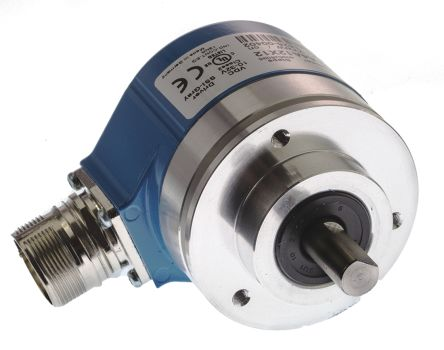
\includegraphics[width=.2\textwidth,height=.3\textheight,keepaspectratio]{images/codeur_optique}
		\end{center}

			Un \textbf{codeur optique} renvoie \textit{un signal carré} dont les caractéristiques permettent de connaitre la position et/ou la vitesse d'un moteur.
		\end{minipage}

		\UPSTIquestion{De quel type (analogique, numérique ou logique) est la sonde de température ci-dessous ?}

		\UPSTIlignesACompleter[1]{Analogique car tension continue image d'une température. }

			\begin{minipage}[b]{.9\textwidth}
			\begin{center}
				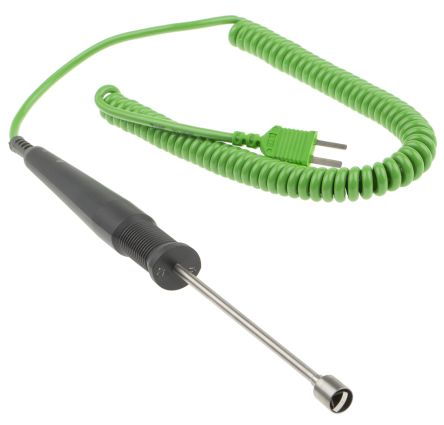
\includegraphics[width=.2\textwidth,height=.3\textheight,keepaspectratio]{images/sondeTemperature}
			\end{center}

				Une \textbf{sonde de température} renvoie \textit{un courant ou une tension} variant de $V_{\text{min}}$ à  $V_{\text{max}}$ en fonction de la température.
			\end{minipage}
\end{UPSTIactivite}

\subsection{Les actionneurs}
Un actionneur est un composant réalisant une conversion d'énergie afin d'agir sur le système. C'est lui qui réalise l'\textbf{action} du système, d'où son nom \textbf{actionneur}.

\UPSTIexemple{%
\begin{minipage}[b]{.49\textwidth}
\centering
	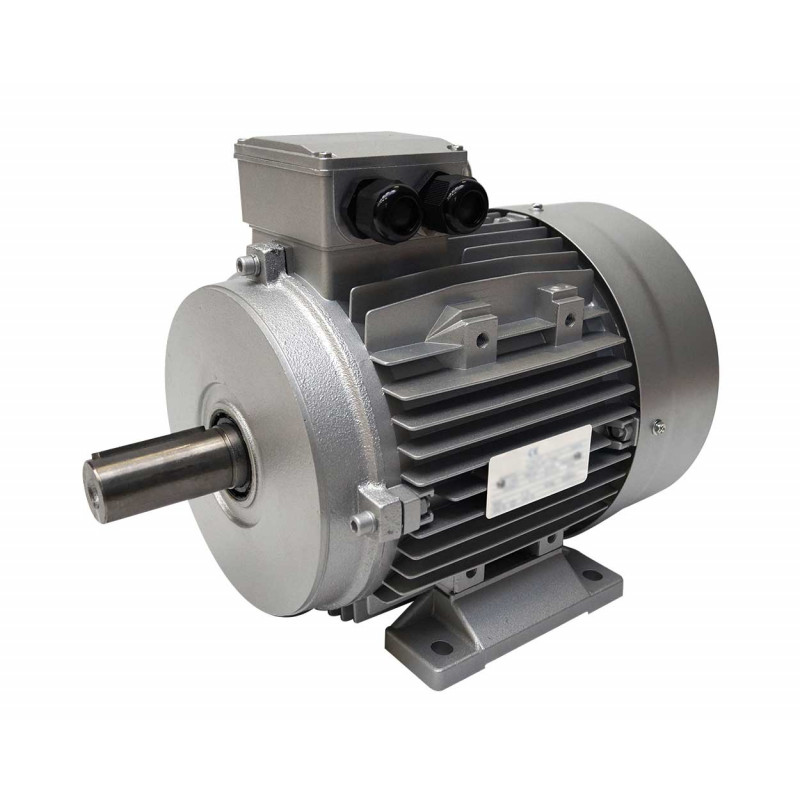
\includegraphics[width=.3\textwidth,height=.4\textheight,keepaspectratio]{images/moteur_electrique_triphase}

	Le moteur à courant continu converti l'énergie électrique en énergie mécanique.
\end{minipage}\hfill
\begin{minipage}[b]{.49\textwidth}
\centering
	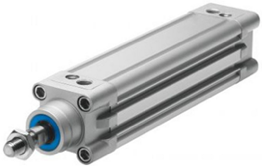
\includegraphics[width=.3\textwidth,height=.4\textheight,keepaspectratio]{images/verin_pneu}

	Un vérin pneumatique converti une énergie pneumatique en énergie mécanique.
\end{minipage}
 %
}

\UPSTIremarque{Les actionneurs ne sont généralement pas reliés directement à l'automate. Un pré-actionneur fait le lien et adapte l'énergie pour l'actionneur.}
)
\subsection{Les pré-actionneurs}
Les \textbf{pré-actionneurs} remplissent la fonction \textit{distribuer} de la chaîne d'énergie. Ce sont eux qui  adaptent l'énergie puis la distribuent aux différents actionneurs. Ils \textbf{sont commandés par l'automate en vue de faire fonctionner les actionneurs}.

\UPSTIaRetenir{Un automate programmable \textbf{commande les pré-actionneurs} pour faire fonctionner les \textit{actionneurs}.}

\UPSTIexemple{%
\begin{minipage}[b]{.49\textwidth}
\centering
	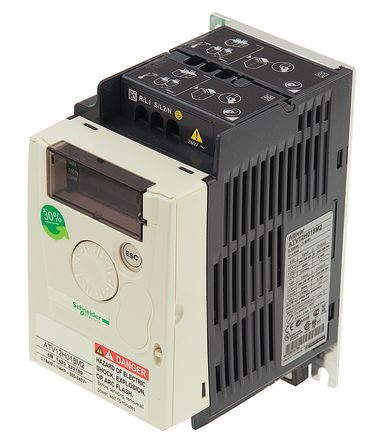
\includegraphics[width=.3\textwidth,height=.4\textheight,keepaspectratio]{images/varia_vitesse_mot_elec}

	Un variateur de vitesse pour moteur électrique adapte la tension d'alimentation du moteur pour en régler la vitesse.
\end{minipage}\hfill
\begin{minipage}[b]{.49\textwidth}
\centering
	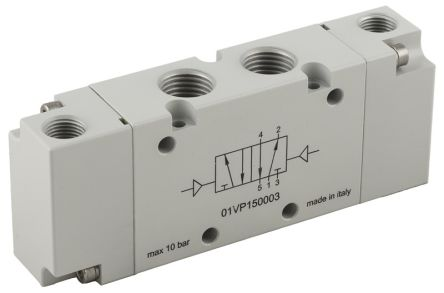
\includegraphics[width=.3\textwidth,height=.4\textheight,keepaspectratio]{images/distri_electroPneu}

	Un distributeur électro-pneumatique contrôle l'arrivée d'air comprimé dans les organes pneumatiques (vérin par exemple).
\end{minipage}
 %
}

\subsection{Interfaces Homme/Machine (IHM)}
L'interface Homme/Machine regroupe les équipements permettant la communication entre l'automate et l'opérateur.

 Elle permet à l'opérateur de communiquer avec le système :
 \begin{description}
   \item [Envoi] de consignes (marche, vitesse de consigne, arrêt, température de consigne, \dots)
   \item [Retour] d'informations sur l'état de la machine (température actuelle, vitesses). L'état actuel du processus (démarrage, remplissage, \dots).
 \end{description}

 Une IHM est généralement composée de \textbf{voyants}, \textbf{boutons poussoirs}, \textbf{écrants} (Figure~\ref{fig:IHM})


\begin{figure}
  \begin{subfigure}{0.49\textwidth}
    \centering
    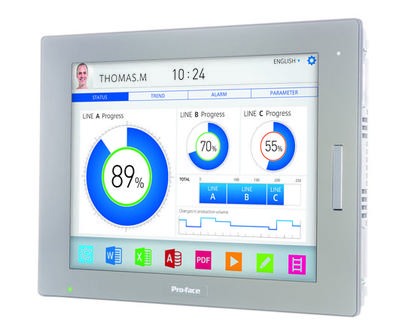
\includegraphics[width=\linewidth, height=.15\textheight,keepaspectratio]{images/ecranIHM}
  \end{subfigure}%
%
  \begin{subfigure}{0.49\textwidth}
    \centering
    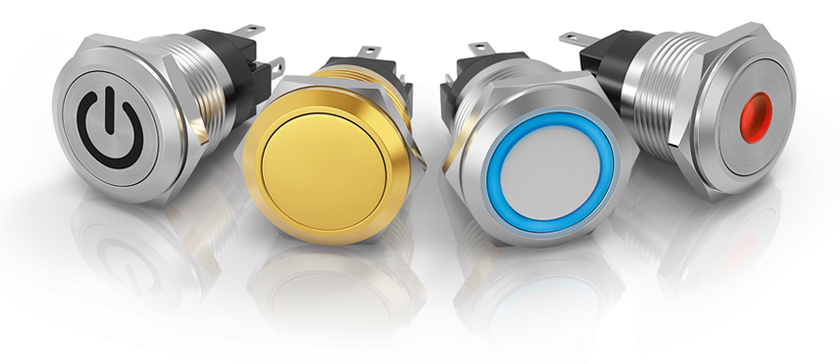
\includegraphics[width=\linewidth,height=.15\textheight,keepaspectratio]{images/boutons}
  \end{subfigure}
  \caption{Ecran et boutons poussoirs pour une IHM}
  \label{fig:IHM}
\end{figure}

%\subsection{Strucure locale et distribuée}
Comme nous l'avons vu dans la section précédente, les automates industriels sont reliés aux capteurs et pré-actionneurs du système.

Sur les systèmes de petite taille et si l'installation le permet, les entrées et sorties de l'automate sont reliées directement à l'automate, on parle de \textbf{structure locale}. Pour des installations plus grande ou lorsque la configuration l'impose, les entrées et sorties sont reliées à des modules déportés (éloignés de l'automate), on parle de \textbf{structure déportée} ou de \textbf{structure distribuée}. Ces deux configurations sont illustrée sur la Figure~\ref{fig:local_deporte}

\begin{figure}[h]
	\begin{subfigure}[b]{.49\textwidth}
		\centering
		


\tikzset{every picture/.style={line width=0.75pt}} %set default line width to 0.75pt

\begin{tikzpicture}[x=0.75pt,y=0.75pt,yscale=-1,xscale=1]
%uncomment if require: \path (0,300); %set diagram left start at 0, and has height of 300

%Image [id:dp060131966756508004]
\draw (75,57) node  {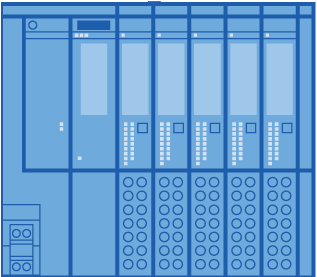
\includegraphics[width=52.5pt,height=52.5pt]{images/siemens_schema.png}};
%Rounded Rect [id:dp7545427239837935]
\draw   (47,129.03) .. controls (47,124.59) and (50.59,121) .. (55.03,121) -- (120.57,121) .. controls (125.01,121) and (128.6,124.59) .. (128.6,129.03) -- (128.6,153.11) .. controls (128.6,157.54) and (125.01,161.13) .. (120.57,161.13) -- (55.03,161.13) .. controls (50.59,161.13) and (47,157.54) .. (47,153.11) -- cycle ;
%Straight Lines [id:da21237841433953675]
\draw [color={rgb, 255:red, 65; green, 117; blue, 5 }  ,draw opacity=1 ]   (71,92) -- (71,119) ;
\draw [shift={(71,121)}, rotate = 270] [color={rgb, 255:red, 65; green, 117; blue, 5 }  ,draw opacity=1 ][line width=0.75]    (10.93,-3.29) .. controls (6.95,-1.4) and (3.31,-0.3) .. (0,0) .. controls (3.31,0.3) and (6.95,1.4) .. (10.93,3.29)   ;

%Straight Lines [id:da9289871961779934]
\draw [color={rgb, 255:red, 208; green, 2; blue, 27 }  ,draw opacity=1 ]   (66,121) -- (66,94) ;
\draw [shift={(66,92)}, rotate = 450] [color={rgb, 255:red, 208; green, 2; blue, 27 }  ,draw opacity=1 ][line width=0.75]    (10.93,-3.29) .. controls (6.95,-1.4) and (3.31,-0.3) .. (0,0) .. controls (3.31,0.3) and (6.95,1.4) .. (10.93,3.29)   ;

%Straight Lines [id:da38366242506499526]
\draw [color={rgb, 255:red, 65; green, 117; blue, 5 }  ,draw opacity=1 ]   (104,92) -- (104,119) ;
\draw [shift={(104,121)}, rotate = 270] [color={rgb, 255:red, 65; green, 117; blue, 5 }  ,draw opacity=1 ][line width=0.75]    (10.93,-3.29) .. controls (6.95,-1.4) and (3.31,-0.3) .. (0,0) .. controls (3.31,0.3) and (6.95,1.4) .. (10.93,3.29)   ;

%Straight Lines [id:da1458665129852148]
\draw [color={rgb, 255:red, 208; green, 2; blue, 27 }  ,draw opacity=1 ]   (99,121) -- (99,94) ;
\draw [shift={(99,92)}, rotate = 450] [color={rgb, 255:red, 208; green, 2; blue, 27 }  ,draw opacity=1 ][line width=0.75]    (10.93,-3.29) .. controls (6.95,-1.4) and (3.31,-0.3) .. (0,0) .. controls (3.31,0.3) and (6.95,1.4) .. (10.93,3.29)   ;


%Straight Lines [id:da7281946578898251]
\draw [color={rgb, 255:red, 65; green, 117; blue, 5 }  ,draw opacity=1 ]   (88.5,92) -- (88.5,119) ;
\draw [shift={(88.5,121)}, rotate = 270] [color={rgb, 255:red, 65; green, 117; blue, 5 }  ,draw opacity=1 ][line width=0.75]    (10.93,-3.29) .. controls (6.95,-1.4) and (3.31,-0.3) .. (0,0) .. controls (3.31,0.3) and (6.95,1.4) .. (10.93,3.29)   ;

%Straight Lines [id:da7853722611490053]
\draw [color={rgb, 255:red, 208; green, 2; blue, 27 }  ,draw opacity=1 ]   (83.5,121) -- (83.5,94) ;
\draw [shift={(83.5,92)}, rotate = 450] [color={rgb, 255:red, 208; green, 2; blue, 27 }  ,draw opacity=1 ][line width=0.75]    (10.93,-3.29) .. controls (6.95,-1.4) and (3.31,-0.3) .. (0,0) .. controls (3.31,0.3) and (6.95,1.4) .. (10.93,3.29)   ;



% Text Node
\draw (87.8,141.07) node  [align=left] {Système};


\end{tikzpicture}

		\caption{Strucure locale}
	\end{subfigure}
	\begin{subfigure}[b]{.49\textwidth}
	\centering
	


\tikzset{every picture/.style={line width=0.75pt}} %set default line width to 0.75pt

\begin{tikzpicture}[x=0.75pt,y=0.75pt,yscale=-1,xscale=1]
%uncomment if require: \path (0,300); %set diagram left start at 0, and has height of 300

%Image [id:dp6138401172065612]
\draw (303,54) node  {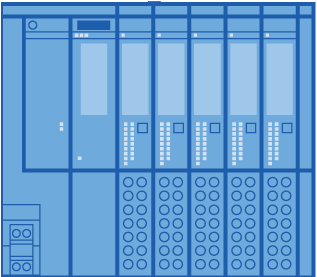
\includegraphics[width=52.5pt,height=52.5pt]{images/siemens_schema.png}};
%Image [id:dp16537534423117606]
\draw (423,74) node  {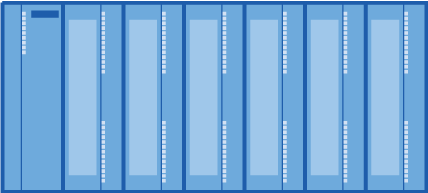
\includegraphics[width=52.5pt,height=25.5pt]{images/entree_sortie_schema.png}};
%Curve Lines [id:da9047126032159685]
\draw [color={rgb, 255:red, 245; green, 166; blue, 35 }  ,draw opacity=1 ]   (278,88) .. controls (279.98,135.52) and (340.52,114.92) .. (386.61,91.7) ;
\draw [shift={(388,91)}, rotate = 513.06] [color={rgb, 255:red, 245; green, 166; blue, 35 }  ,draw opacity=1 ][line width=0.75]    (10.93,-3.29) .. controls (6.95,-1.4) and (3.31,-0.3) .. (0,0) .. controls (3.31,0.3) and (6.95,1.4) .. (10.93,3.29)   ;

%Rounded Rect [id:dp33312095954877385]
\draw   (381,128.03) .. controls (381,123.59) and (384.59,120) .. (389.03,120) -- (454.57,120) .. controls (459.01,120) and (462.6,123.59) .. (462.6,128.03) -- (462.6,152.11) .. controls (462.6,156.54) and (459.01,160.13) .. (454.57,160.13) -- (389.03,160.13) .. controls (384.59,160.13) and (381,156.54) .. (381,152.11) -- cycle ;
%Straight Lines [id:da4805908792581848]
\draw [color={rgb, 255:red, 65; green, 117; blue, 5 }  ,draw opacity=1 ]   (405,91) -- (405,118) ;
\draw [shift={(405,120)}, rotate = 270] [color={rgb, 255:red, 65; green, 117; blue, 5 }  ,draw opacity=1 ][line width=0.75]    (10.93,-3.29) .. controls (6.95,-1.4) and (3.31,-0.3) .. (0,0) .. controls (3.31,0.3) and (6.95,1.4) .. (10.93,3.29)   ;

%Straight Lines [id:da046732551722878934]
\draw [color={rgb, 255:red, 208; green, 2; blue, 27 }  ,draw opacity=1 ]   (400,120) -- (400,93) ;
\draw [shift={(400,91)}, rotate = 450] [color={rgb, 255:red, 208; green, 2; blue, 27 }  ,draw opacity=1 ][line width=0.75]    (10.93,-3.29) .. controls (6.95,-1.4) and (3.31,-0.3) .. (0,0) .. controls (3.31,0.3) and (6.95,1.4) .. (10.93,3.29)   ;

%Straight Lines [id:da5001732327017756]
\draw [color={rgb, 255:red, 65; green, 117; blue, 5 }  ,draw opacity=1 ]   (438,91) -- (438,118) ;
\draw [shift={(438,120)}, rotate = 270] [color={rgb, 255:red, 65; green, 117; blue, 5 }  ,draw opacity=1 ][line width=0.75]    (10.93,-3.29) .. controls (6.95,-1.4) and (3.31,-0.3) .. (0,0) .. controls (3.31,0.3) and (6.95,1.4) .. (10.93,3.29)   ;

%Straight Lines [id:da6761611930473217]
\draw [color={rgb, 255:red, 208; green, 2; blue, 27 }  ,draw opacity=1 ]   (433,120) -- (433,93) ;
\draw [shift={(433,91)}, rotate = 450] [color={rgb, 255:red, 208; green, 2; blue, 27 }  ,draw opacity=1 ][line width=0.75]    (10.93,-3.29) .. controls (6.95,-1.4) and (3.31,-0.3) .. (0,0) .. controls (3.31,0.3) and (6.95,1.4) .. (10.93,3.29)   ;


%Straight Lines [id:da5215523224998694]
\draw [color={rgb, 255:red, 65; green, 117; blue, 5 }  ,draw opacity=1 ]   (422.5,91) -- (422.5,118) ;
\draw [shift={(422.5,120)}, rotate = 270] [color={rgb, 255:red, 65; green, 117; blue, 5 }  ,draw opacity=1 ][line width=0.75]    (10.93,-3.29) .. controls (6.95,-1.4) and (3.31,-0.3) .. (0,0) .. controls (3.31,0.3) and (6.95,1.4) .. (10.93,3.29)   ;

%Straight Lines [id:da15501163618778613]
\draw [color={rgb, 255:red, 208; green, 2; blue, 27 }  ,draw opacity=1 ]   (417.5,120) -- (417.5,93) ;
\draw [shift={(417.5,91)}, rotate = 450] [color={rgb, 255:red, 208; green, 2; blue, 27 }  ,draw opacity=1 ][line width=0.75]    (10.93,-3.29) .. controls (6.95,-1.4) and (3.31,-0.3) .. (0,0) .. controls (3.31,0.3) and (6.95,1.4) .. (10.93,3.29)   ;




% Text Node
\draw (304,126) node [scale=0.9,color={rgb, 255:red, 245; green, 166; blue, 35 }  ,opacity=1 ] [align=left] {Bus de terrain};
% Text Node
\draw (421.8,140.07) node  [align=left] {Système};


\end{tikzpicture}

	\caption{Strucure distribuée}
	\end{subfigure}
	\caption{Schéma de structure locale et déportée}
	\label{fig:local_deporte}
\end{figure}

Les bus de terrain reliant les modules peuvent être de différentes natures selon la configuration (CAN, Profibus, LON, BACNET, Ethernet, \dots).

\UPSTIaRetenir{%
\begin{description}
	\item [Sructure locale : ] Les modules d'entrées et de sorties sont reliées directements à l'automate.
	\item [Strucure déportée : ] Les modules d'entrées et de sorties sont déportées proches des capteurs et actionneurs et communiquent avec l'automates à l'aide d'un BUS de terrain.
\end{description}
}

